\documentclass[a4paper]{article}

%% Language and font encodings
\usepackage[english]{babel}
\usepackage[utf8x]{inputenc}
\usepackage[T1]{fontenc}

%% Sets page size and margins
\usepackage[a4paper,top=3cm,bottom=2cm,left=3cm,right=3cm,marginparwidth=1.75cm]{geometry}

%% Useful packages
\usepackage{amsmath}
\usepackage{graphicx}
\usepackage[colorinlistoftodos]{todonotes}
\usepackage[colorlinks=true, allcolors=blue]{hyperref}

\title{Neo4j math-search attempt}
\author{Wei Zhong}

\begin{document}
\maketitle

\section{Neo4j auto-complete method}
We want to know if any frequency/usability criteria is used for Neo4j completions. I have looked \cite{officialsite, github, se, github_src} and I get to know the autocomplete facility is provided as a ``shell" function to Neo4j query input \cite{github_src}. But I think the focus of Neo4j GUI is not on auto-completion, there is no dedicated documentation on how Neo4j autocompletion works. And after spending a lot of time searching the document/code, I cannot find whether or not they have used frequency to rank autocomplete candidates.

\section{Imitate math-search using Neo4j}
First clear the database,
\begin{verbatim}
match (n) detach delete n
\end{verbatim}
We can add paths into graph by adding token node pairs along the path:
\begin{verbatim}
merge (t1:Token {name: "VAR"})
merge (t2:Token {name: "TIMES"})
merge (t1)-[r:under]->(t2)
return t1,r,t2
\end{verbatim}
The ``merge'' command will check if there is any existing token node with same name, it will add the node of that token only if it cannot find any existing token of same name. 
But this operation is not what we need, because when it cannot find existing nodes/path, it will create a duplicate one where in our case the common prefix of two paths are supposed to be merged (diverge on some node).
\begin{figure}
\centering
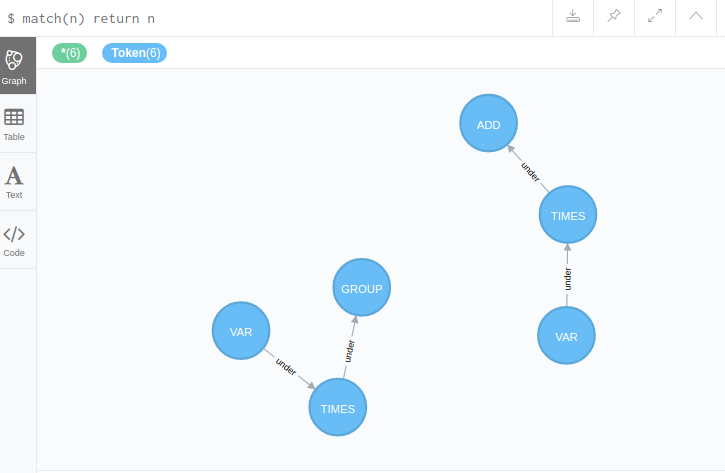
\includegraphics[width=1.0\textwidth]{fig1.png}
\caption{\label{fig1}Not be able to merge paths}
\end{figure}

For example, if you input two paths using merge command:
\begin{verbatim}
match (n) detach delete n

merge
(:Token{name:"VAR"})-[:under]->
(:Token{name:"TIMES"})-[:under]->
(:Token{name:"ADD"})

merge
(:Token{name:"VAR"})-[:under]->
(:Token{name:"TIMES"})-[:under]->
(:Token{name:"GROUP"})

match(n) return n
\end{verbatim}
There will be two paths instead of one diverged branch (see Figure~\ref{fig1}).

So far the only way I know to insert path into tree without creating duplicate path is progressively match the path prefix until the last node is not existing, and you insert the rest of nodes at that point, something like below to find the node to append after:
\begin{verbatim}
MATCH
path = (Token{name:"VAR"})-[:under]->
(Token{name:"TIMES"})-[:under]->
(Token{name:"ADD"})
return path

(no changes, no records)

MATCH
(Token{name:"VAR"})-[:under]->
(t2:Token{name:"TIMES"})
CREATE (t2)-[:under]->(:Token{name:"ADD"})
\end{verbatim}

\begin{figure}
\centering
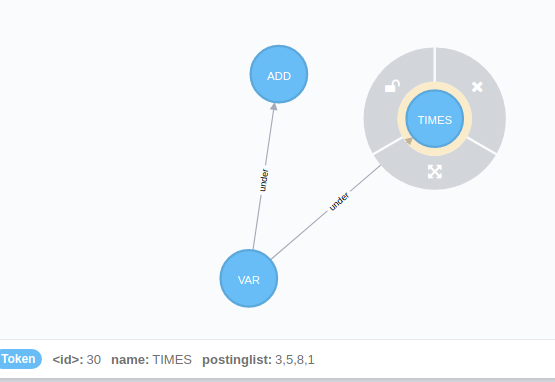
\includegraphics[width=1.0\textwidth]{fig2.png}
\caption{\label{fig2}Posting list imitation}
\end{figure}

For posting list, below is the way to imitate appending document ID to particular posting list by first finding the node who contains the posting list property (array) to push new document ID.
\begin{verbatim}
match (n) detach delete n

MERGE
(:Token{name:"VAR"})-[:under]->
(:Token{name:"TIMES", postinglist: []})

MATCH
(t:Token{name:"VAR"})
CREATE (t)-[:under]->(:Token{name:"ADD", postinglist: []})

MATCH
(Token{name:"VAR"})-[:under]->
(t:Token{name:"TIMES"})
SET t.postinglist = t.postinglist + [3]

...
\end{verbatim}
The resulting graph looks like see Figure~\ref{fig2}.

To intersect the posting list,
\begin{verbatim}
MATCH
(:Token{name:"VAR"})-[:under]->
(t1:Token{name:"TIMES"}),
(:Token{name:"VAR"})-[:under]->
(t2:Token{name:"ADD"})
RETURN apoc.coll.intersection(t1.postinglist, t2.postinglist) as results
\end{verbatim}

Now we have imitated all the very basic components of how Approach0 deals with math indexing and searching, but inserting paths like this way is far too tedious to write it by hand for even a small collection. This is the major problem to index a corpus into Neo4j graph database, what we need now is a procedure and ``for loop'' to actually program the way Approach0 indexes a path without issuing too many commands by hand, after many attempts, I failed to do this in a Neo4j procedure: 
\begin{verbatim}
with {path: ["VAR", "GROUP"]} as j
unwind j.path as node
return node
\end{verbatim}

\begin{verbatim}
with {path: ["VAR", "GROUP"]} as j
unwind j.path as nodes
foreach (n in nodes |
	MATCH (Token{name:n})-[:under]->(t:Token{name:"TIMES"})
)

Neo.ClientError.Statement.SyntaxError
Invalid use of MATCH inside FOREACH (line 4, column 2 (offset: 81))
"	MATCH (Token{name:n})-[:under]->(t:Token{name:"TIMES"})"
  ^
\end{verbatim}

\bibliographystyle{abbrv}
\bibliography{sample}

\end{document}
